%%%%%%%%%%%%%%%%%%%%%%%%%%%%%%%%%%%%%%%%%%%%%%%%%%%%%%%%%%%%%%%%%%%%%%%%%%%%%%%%
%%%%%%%%%%%%%%%%%%%%%%%%%%%%%%%%%%%%%%%%%%%%%%%%%%%%%%%%%%%%%%%%%%%%%%%%%%%%%%%%
%%% Template for AIMS Rwanda Assignments         %%%              %%%
%%% Author:   AIMS Rwanda tutors                             %%%   ###        %%%
%%% Email: tutors2017-18@aims.ac.rw                               %%%   ###        %%%
%%% Copyright: This template was designed to be used for    %%% #######      %%%
%%% the assignments at AIMS Rwanda during the academic year %%%   ###        %%%
%%% 2017-2018.                                              %%%   #########  %%%
%%% You are free to alter any part of this document for     %%%   ###   ###  %%%
%%% yourself and for distribution.                          %%%   ###   ###  %%%
%%%                                                         %%%              %%%
%%%%%%%%%%%%%%%%%%%%%%%%%%%%%%%%%%%%%%%%%%%%%%%%%%%%%%%%%%%%%%%%%%%%%%%%%%%%%%%%
%%%%%%%%%%%%%%%%%%%%%%%%%%%%%%%%%%%%%%%%%%%%%%%%%%%%%%%%%%%%%%%%%%%%%%%%%%%%%%%%


%%%%%% Ensure that you do not write the questions before each of the solutions because it is not necessary. %%%%%% 

\documentclass[12pt,a4paper]{article}

%%%%%%%%%%%%%%%%%%%%%%%%% packages %%%%%%%%%%%%%%%%%%%%%%%%
\usepackage{amsmath}
\usepackage{amssymb}
\usepackage{amsthm}
\usepackage{amsfonts}
\usepackage{graphicx}
\usepackage[all]{xy}
\usepackage{actuarialsymbol}
\usepackage{actuarialangle}
\usepackage{tikz}
\usepackage{verbatim}
\usepackage[left=2cm,right=2cm,top=3cm,bottom=2.5cm]{geometry}
\usepackage{hyperref}
\usepackage{caption}
\usepackage{subcaption}
\usepackage{psfrag}

%%%%%%%%%%%%%%%%%%%%% students data %%%%%%%%%%%%%%%%%%%%%%%%
\newcommand{\student}{Akor Stanley}
\newcommand{\course}{NM1 }
\newcommand{\assignment}{1}

%%%%%%%%%%%%%%%%%%% using theorem style %%%%%%%%%%%%%%%%%%%%
\newtheorem{thm}{Theorem}
\newtheorem{lem}[thm]{Lemma}
\newtheorem{defn}[thm]{Definition}
\newtheorem{exa}[thm]{Example}
\newtheorem{rem}[thm]{Remark}
\newtheorem{coro}[thm]{Corollary}
\newtheorem{quest}{Question}[section]

%%%%%%%%%%%%%%  Shortcut for usual set of numbers  %%%%%%%%%%%

\newcommand{\N}{\mathbb{N}}
\newcommand{\Z}{\mathbb{Z}}
\newcommand{\Q}{\mathbb{Q}}
\newcommand{\R}{\mathbb{R}}
\newcommand{\C}{\mathbb{C}}
%%%%%%%%%%%%%%%%%%%%%%%%%%%%%%%%%%%%%%%%%%%%%%%%%%%%%%%555
\begin{document}
%%%%%%%%%%%%%%%%%%%%%%% title page %%%%%%%%%%%%%%%%%%%%%%%%%%
\thispagestyle{empty}
\begin{center}
\textbf{AFRICAN INSTITUTE FOR MATHEMATICAL SCIENCES \\[0.5cm]
(AIMS RWANDA, KIGALI)}
\vspace{1.0cm}
\end{center}
%%%%%%%%%%%%%%%%%%%%% assignment information %%%%%%%%%%%%%%%%
\noindent
\rule{17cm}{0.2cm}\\[0.3cm]
Name: \student \hfill Assignment Number: \assignment\\[0.1cm]
Course: \course \hfill Date: \today\\
\rule{17cm}{0.05cm}
\vspace{1.0cm}
\section*{Question 1}
\begin{align*}
\begin{cases}
v^{\prime \prime \prime}(t)=v(t)v^{\prime}-s(t)(v^{\prime \prime}(t))^{2}, \quad \forall t>0\\
v(0)=1, \quad v^{\prime}(0)=0; \quad v^{\prime \prime}(0)=2
\end{cases}
\end{align*}
Where $s(t)$ is a given function.
\begin{itemize}
	\item [(1)]
	We start by re-writing the given equation as a system of first order ordinary differential equations
	\begin{align*}
	\begin{cases}
	v^{\prime}(t)=x(t)\\
	x^{\prime}(t)=y(t)\\
	y^{\prime}(t)=v(t)x(t)-s(t)(y(t))^{2}
	\end{cases}
	\end{align*}
	Let;
	\begin{align}
	\textbf{Y}(t)&=\begin{pmatrix}
	v\\x\\y
	\end{pmatrix}\implies \textbf{Y}^{\prime}(t)= \begin{pmatrix}
	v^{\prime}\\
	x^{\prime}\\
	y^{\prime}
	\end{pmatrix}=\begin{pmatrix}
	x\\
	y\\
	vx-sy^{2}
	\end{pmatrix} \label{1}
	\end{align}
	Thus;
	\begin{align*}
	F(t,\textbf{Y})=\begin{pmatrix}
	x\\
	y\\
	vx-sy^{2}
	\end{pmatrix} 
	\end{align*}
	Where
	\begin{align*}
	\textbf{Y(0)}=\textbf{Y}_{\circ}=\begin{pmatrix}
	1\\0\\2
	\end{pmatrix}
	\end{align*}
	Therefore;
	\begin{align*}
	\textbf{Y}^{\prime}(t)=	F(t,\textbf{Y})
	\end{align*}
	\item[(2)] The associated midpoint is given by;\\
	%$v_{1}\approx v(t_{1})$\\
	$v(0)=v_{\circ}$\\
	$x(0)=x_{\circ}$\\
	$y(0)=y_{\circ}$\\
	$\Delta t_{n}=\Delta t$\\
	$t_{n}=t_{\circ}+n\Delta t$\\
	$t_{n+\frac{1}{2}}=t_{n}+\frac{\Delta t}{2}$\\
	$\textbf{Y}_{n+\frac{1}{2}}=\textbf{Y}_{n}+\frac{\Delta t}{2}F(t_{n},\textbf{Y}_{n})$\\
	$\textbf{Y}_{n+1}=\textbf{Y}_{n}+\Delta tF(t_{n+\frac{1}{2}},\textbf{Y}_{n+\frac{1}{2}})$
	\item [(3)]
	
	Kindly note that I made a change of variable from the initial vector \textbf{Y}$_{n}$ in equation\ref{1} to \textbf{V}$_{n}$ in order to be consistent with the requirements of the given problem.
	\begin{align*}
	\begin{cases}
	t_{\circ}=0\\
	\Delta t=0.5\\
	s=1+t^{2}
	\end{cases}
	\end{align*}
	For $n=0$;
	\begin{align*}
	t_{n+\frac{1}{2}}&=t_{n}+\frac{\Delta t}{2}\\ t_{\frac{1}{2}}&=t_{\circ}+\frac{0.5}{2}=0.25
	\end{align*}
	\begin{align*}
	\textbf{V}_{\frac{1}{2}}&=\textbf{V}_{\circ}+ \frac{\Delta t}{2}F(t_{\circ},\textbf{V}_{\circ})\\
	\textbf{V}_{\frac{1}{2}}&=\begin{pmatrix}
	1\\0\\2
	\end{pmatrix} + 0.25\begin{pmatrix}
	x_{\circ}\\
	y_{\circ}\\
	v_{\circ}x_{\circ}-(1+t_{\circ}^{2})y_{\circ}^{2}
	\end{pmatrix}\\
	\textbf{V}_{\frac{1}{2}}&=\begin{pmatrix}
	1\\0\\2
	\end{pmatrix} + 0.25\begin{pmatrix}
	0\\2\\-4
	\end{pmatrix}\\
	\textbf{V}_{\frac{1}{2}}&=\begin{pmatrix}
	1\\
	0.5\\
	1
	\end{pmatrix}
	\end{align*}
	\begin{align*}
	\textbf{V}_{n+1}&=\textbf{v}_{n}+\Delta F(t_{n+\frac{1}{2}},\textbf{V}_{n+\frac{1}{2}})\\
	\textbf{V}_{1}&=\textbf{v}_{\circ}+ \Delta F(t_{\frac{1}{2}},\textbf{V}_{\frac{1}{2}})\\
	\textbf{V}_{1}&=\begin{pmatrix}
	1\\0\\2
	\end{pmatrix}+0.5\begin{pmatrix}
	0.5\\
	1\\
	0.5\times 1-(1+0.25^{2})\times 1 
	\end{pmatrix}\\
	\textbf{V}_{1}&=\begin{pmatrix}
	1\\0\\2
	\end{pmatrix} + \begin{pmatrix}
	0.25\\
	0.5\\
	-0.28125
	\end{pmatrix}=\begin{pmatrix}
	1.25\\
	0.5\\
	1.71875
	\end{pmatrix}
	\end{align*}
	$v_{1}=1.25$\\
	\newline
	For $n=1$
	\begin{align*}
	t_{\frac{3}{2}}&=t_{1}+\frac{\Delta t}{2}=0.5+0.25=0.75\\
	\textbf{V}_{\frac{3}{2}}&=\textbf{V}_{1}+\frac{\Delta t}{2} F(t_{1}, \textbf{V}_{1})\\
	&=\begin{pmatrix}
	1.25\\
	0.5\\
	1.71875
	\end{pmatrix} +0.25\begin{pmatrix}
	0.5\\
	1.71875\\
	1.25 \times 0.5-(1+0.5^{2})1.71875^{2}
	\end{pmatrix}\\
	&=\begin{pmatrix}
	1.25\\
	0.5\\
	1.71875
	\end{pmatrix} + \begin{pmatrix}
	0.125\\
	0.42968\\
	-0.7669	
	\end{pmatrix}\\
\textbf{V}_{\frac{3}{2}}	&=\begin{pmatrix}
	1.375\\
	0.92968\\
	0.9518
	\end{pmatrix}
	\end{align*}
	\begin{align*}
	\textbf{V}_{2}&=\textbf{v}_{1}+\Delta t F(t_{\frac{3}{2}},\textbf{V}_{\frac{3}{2}})\\
	\textbf{V}_{2}&=\begin{pmatrix}
	1.25\\
	0.5\\
	1.71875
	\end{pmatrix} +0.5\begin{pmatrix}
	0.92968\\
	0.9518\\
	1.375\times 0.92968-(1+0.75^{2})0.9518^{2}\\
	\end{pmatrix}\\
	&=\begin{pmatrix}
	1.25\\
	0.5\\
	1.71875
	\end{pmatrix} + \begin{pmatrix}
	0.46484\\
	0.4759\\
	-0.06859
	\end{pmatrix}\\
	\textbf{V}_{2}&=\begin{pmatrix}
	1.7148\\
	0.9759\\
	1.65016
	\end{pmatrix}
	\end{align*}
	$v_{2}=1.7148$
\end{itemize}
\newpage
\section*{Question 2}
Given;
\begin{align}
C\frac{dT}{dt}=\frac{(1-\alpha)S_{\circ}}{4}-\epsilon\sigma T^{4} \label{2}
\end{align}
Where: $C=85,\quad \alpha=0.3, \quad S_{\circ}=1367, \epsilon=0.6, \sigma =5.67\times 10^{-8}$ and $T=T(t)$ is the globally averaged surface temperature.
\begin{itemize}
	\item [(1)] At equilibruim temperature $T_{eq}$, $\frac{dT}{dt}=0$, thus equation\ref{2} becomes;
	\begin{align*}
	C\times 0&=\frac{(1-\alpha)S_{\circ}}{4}-\epsilon\sigma T^{4}_{eq}\\
	T^{4}_{eq}&=\frac{(1-\alpha)S_{\circ}}{4\epsilon\sigma}\\
	T_{eq}&=\sqrt[4]{\frac{(1-\alpha)S_{\circ}}{4\epsilon\sigma}}\\
	&=\sqrt[4]{\frac{(1-0.3)1367}{4\times 0.6\times 5.67\times 10^{-8} }}\\
	&=289.57K
	\end{align*}
	Therefore, $T_{eq}=289.57K$
	\item[(2)] We want to show that;
	\begin{align}
	C\frac{dT}{dt}=\frac{(1-\alpha)S_{\circ}}{4}-\epsilon\sigma	T^{4} \label{3}
	\end{align}
	Where; $T(t)=T_{eq}+\tilde{T}(t)$, by substituting $T(t)$ in equation\ref{3}, we shall have;
	\begin{align*}
	C\frac{d(T_{eq}+\tilde{T}(t))}{dt}&=\frac{(1-\alpha)S_{\circ}}{4}-\epsilon\sigma(\tilde{T}+T_{eq})^{4}\\
	C\frac{dT_{eq}}{dt}+C\frac{d\tilde{T}}{dt}&=\frac{(1-\alpha)S_{\circ}}{4}-\epsilon\sigma(\tilde{T}+T_{eq})^{4}
	\end{align*}
	At equilibrium, $\frac{dT_{eq}}{dt}=0$, thus;
	\begin{align}
	C\frac{d\tilde{T}}{dt}&=\frac{(1-\alpha)S_{\circ}}{4}-\epsilon\sigma(\tilde{T}+T_{eq})^{4} \label{5}
	\end{align}
	Hence proved!
	\item [(3)] Assume that
	\begin{align}
	\left(1+\frac{\tilde{T}}{T_{eq}}\right)^{4}=1 +4\frac{\tilde{T}}{T_{eq}} \label{6}
	\end{align}
	we are required to prove
	\begin{align*}
	\frac{d\tilde{T}}{dt}=-\left(\frac{4\epsilon\sigma T^{3}_{eq}}{C}\right)\tilde{T}
	\end{align*}
	From equation\ref{5}, we showed that 
	\begin{align*}
	C\frac{d\tilde{T}}{dt}&=\frac{(1-\alpha)S_{\circ}}{4}-\epsilon\sigma(\tilde{T}+T_{eq})^{4} 
	\end{align*}
	we can further simplify it as;
	\begin{align*}
	C\frac{d\tilde{T}}{dt}&=\frac{(1-\alpha)S_{\circ}}{4}-\epsilon\sigma\left(T_{eq}\left(1+\frac{\tilde{T}}{T_{eq}}\right)\right)^{4} \\
	%C\frac{d\tilde{T}}{dt}&=\frac{(1-\alpha)S_{\circ}}{4}-\epsilon\sigma \left(T_{eq}\left(1+\frac{\tilde{T}}{T_{eq}}\right)\right)^{4}\\
	C\frac{d\tilde{T}}{dt}&=\frac{(1-\alpha)S_{\circ}}{4}-\epsilon\sigma T^{4}_{eq}\left(1+\frac{\tilde{T}}{T_{eq}}\right)^{4} 
	\end{align*}
	Using the relation in equation\ref{6}, we get;
	\begin{align*}
	C\frac{d\tilde{T}}{dt}&=\frac{(1-\alpha)S_{\circ}}{4}-\epsilon\sigma T^{4}_{eq}\left(1 +4\frac{\tilde{T}}{T_{eq}}\right)\\
	C\frac{d\tilde{T}}{dt}&=\frac{(1-\alpha)S_{\circ}}{4}-4\epsilon\sigma T^{3}_{eq}\tilde{T}-\epsilon\sigma T^{4}_{eq}
	\end{align*}
	But at equilibrium,
	\begin{align*}
	\epsilon\sigma T^{4}_{eq}&=\frac{(1-\alpha)S_{\circ}}{4}\\	
	\end{align*}
	by substitution, we then have,
	\begin{align*}
	C\frac{d\tilde{T}}{dt}&=\frac{(1-\alpha)S_{\circ}}{4}-4\epsilon\sigma T^{3}_{eq}\tilde{T}-\frac{(1-\alpha)S_{\circ}}{4}\\
	C\frac{d\tilde{T}}{dt}&=-4\epsilon\sigma T^{3}_{eq}\tilde{T}\\
	\frac{d\tilde{T}}{dt}&=-\left(\frac{4\epsilon\sigma T^{3}_{eq}}{C}\right)\tilde{T} \quad \quad  \quad  \quad 2(a)
	\end{align*}
	Hence shown!
	\item [(4)] Given $\tilde{T}(0)=0$, we want to find the exact solution of (2a)
	\begin{align*}
	\frac{d\tilde{T}}{dt}&=-\left(\frac{4\epsilon\sigma T^{3}_{eq}}{C}\right)\tilde{T}\\
	\frac{d\tilde{T}}{\tilde{T}}&=-\left(\frac{4\epsilon\sigma T^{3}_{eq}}{C}\right)dt\\
	\int \frac{d\tilde{T}}{\tilde{T}}&=-\int \left(\frac{4\epsilon\sigma T^{3}_{eq}}{C}\right)dt\\
	\tilde{T}&=\exp\left[\frac{-4\epsilon\sigma T^{3}_{eq}t}{C}\right]+ B\\
	\tilde{T}&=A\exp\left[\frac{-4\epsilon\sigma T^{3}_{eq}t}{C}\right]
	\end{align*}
	$\tilde{T}(0)=10$, thus
	\begin{align*}
	10&=A\exp(0)\\
	A&=10
	\end{align*}
	The exact solution is given as;
	\begin{align*}
	\tilde{T}(t)&=10\exp\left[\frac{-4\epsilon\sigma T^{3}_{eq}t}{C}\right]
	\end{align*}
	By substituting the values of $C$, $\sigma$, $\epsilon$, $T_{eq}$, we shall obtain;
	\begin{align*}
		\tilde{T}(t)&=10\exp[-0.0388t]
	\end{align*}
	\item [(5a)] 
	\begin{align*}
	(P)
	\begin{cases}
	y_{\circ}&=y_{\circ}\\
	K_{1}&=f(t_{n},y_{n})\\
	t_{n+\frac{3}{4}}&=t_{n}+\frac{3}{4} \Delta t\\
	y_{n+\frac{3}{4}}&=y_{n}+\frac{3}{4} \Delta t K_{1}\\
	K_{2}&=f(t_{n+\frac{3}{4}},y_{n+\frac{3}{4}})\\
	y_{n+1}&=y_{n}+\frac{1}{3}\Delta t (K_{1}+2K_{2})
	\end{cases}
	\end{align*}
	For a one step method;
	\begin{align}
	y_{n+1}=y_{n}+\Delta t_{n}\phi(t_{n},y_{n},\Delta t_{n}) \label{7}
	\end{align}
	From the given scheme
	\begin{align*}
	y_{n+1}&=y_{n}+\frac{1}{3}\Delta t (K_{1}+2K_{2})
	\end{align*}
	By substituting for $K_{1}$ and $K_{2}$
	\begin{align*}
		y_{n+1}&=y_{n}+\frac{1}{3}\Delta t \left(f(t_{n},y_{n})+ 2f(t_{n+\frac{3}{4}},y_{n+\frac{3}{4}}) \right)
	\end{align*}
	By substituting for $t_{n+\frac{3}{4}}$ and $y_{n+\frac{3}{4}}$, we obtain;
	\begin{align*}
	y_{n+1}&=y_{n}+ \frac{1}{3}\Delta t\left(f(t_{n},y_{n})+2\left(t_{n}+\frac{3}{4} \Delta t,y_{n}+\frac{3}{4} \Delta t K_{1}\right)\right)
	\end{align*}
	Now substituting for $K_{1}$, we get
	\begin{align}
	y_{n+1}&=y_{n}+ \frac{1}{3}\Delta t\left(f(t_{n},y_{n})+2\left(t_{n}+\frac{3}{4} \Delta t,y_{n}+\frac{3}{4} \Delta t \centerdot f(t_{n},y_{n})\right)\right) \label{8}
	\end{align}
	From equation\ref{6} and equation\ref{8}, we obtain $\phi$
	\begin{align*}
	\phi(t_{n},y_{n},\Delta t_{n})&=\frac{1}{3}\left(f(t_{n},y_{n})+2\left(t_{n}+\frac{3}{4} \Delta t,y_{n}+\frac{3}{4} \Delta t \centerdot f(t_{n},y_{n})\right)\right)
	\end{align*}
	Thus for $u,v,w$
	\begin{align*}
	\phi(u,v,w)&=\frac{1}{3}\left(f(u,v)+2\left(u+\frac{3}{4} w,v+\frac{3}{4} w \centerdot f(u,v)\right)\right)
	\end{align*}
	Where $\phi$ is a continuous function.
	\newpage
	\item[(5b)]
	.\\
	\begin{figure}[h!]
		\centering
		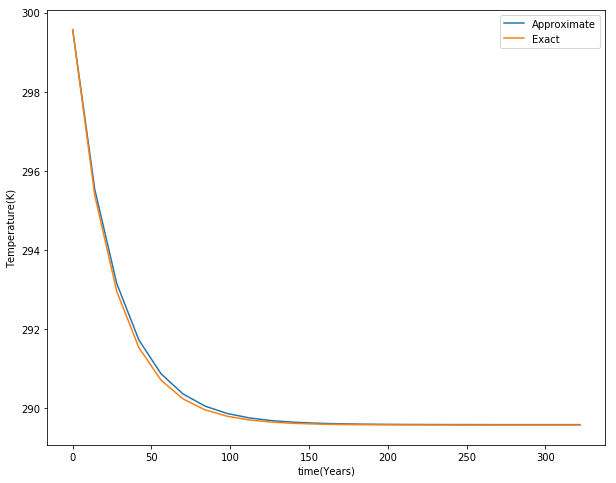
\includegraphics[scale=0.5]{1.png}
		\caption{Exact and Approximate solution}
	\end{figure}
\end{itemize}
\end{document}